\documentclass[12pt]{article}

\usepackage{graphicx}
\usepackage{indentfirst}
\usepackage{tabularx}
\usepackage{caption}
\usepackage{subfigure}
\usepackage{fancyvrb}
\usepackage{listings}
\usepackage[polish, english]{babel}
\usepackage[a4paper, total={16cm, 25cm}]{geometry}
\usepackage[T1]{fontenc}

\usepackage{float}

\floatstyle{ruled}
\newfloat{program}{thp}{lop}
\floatname{program}{Kod}

%opening
\title{\textbf{Specyfikacja modułu exe\_unit\_w6}}
\author{Patryk Korycki, nr albumu 318529}

\begin{document}
	\selectlanguage{polish}{\maketitle}
	
	\label{sec:hello}
	\begin{figure}[!h]
		\begin{center}
			\vspace{-20pt}
			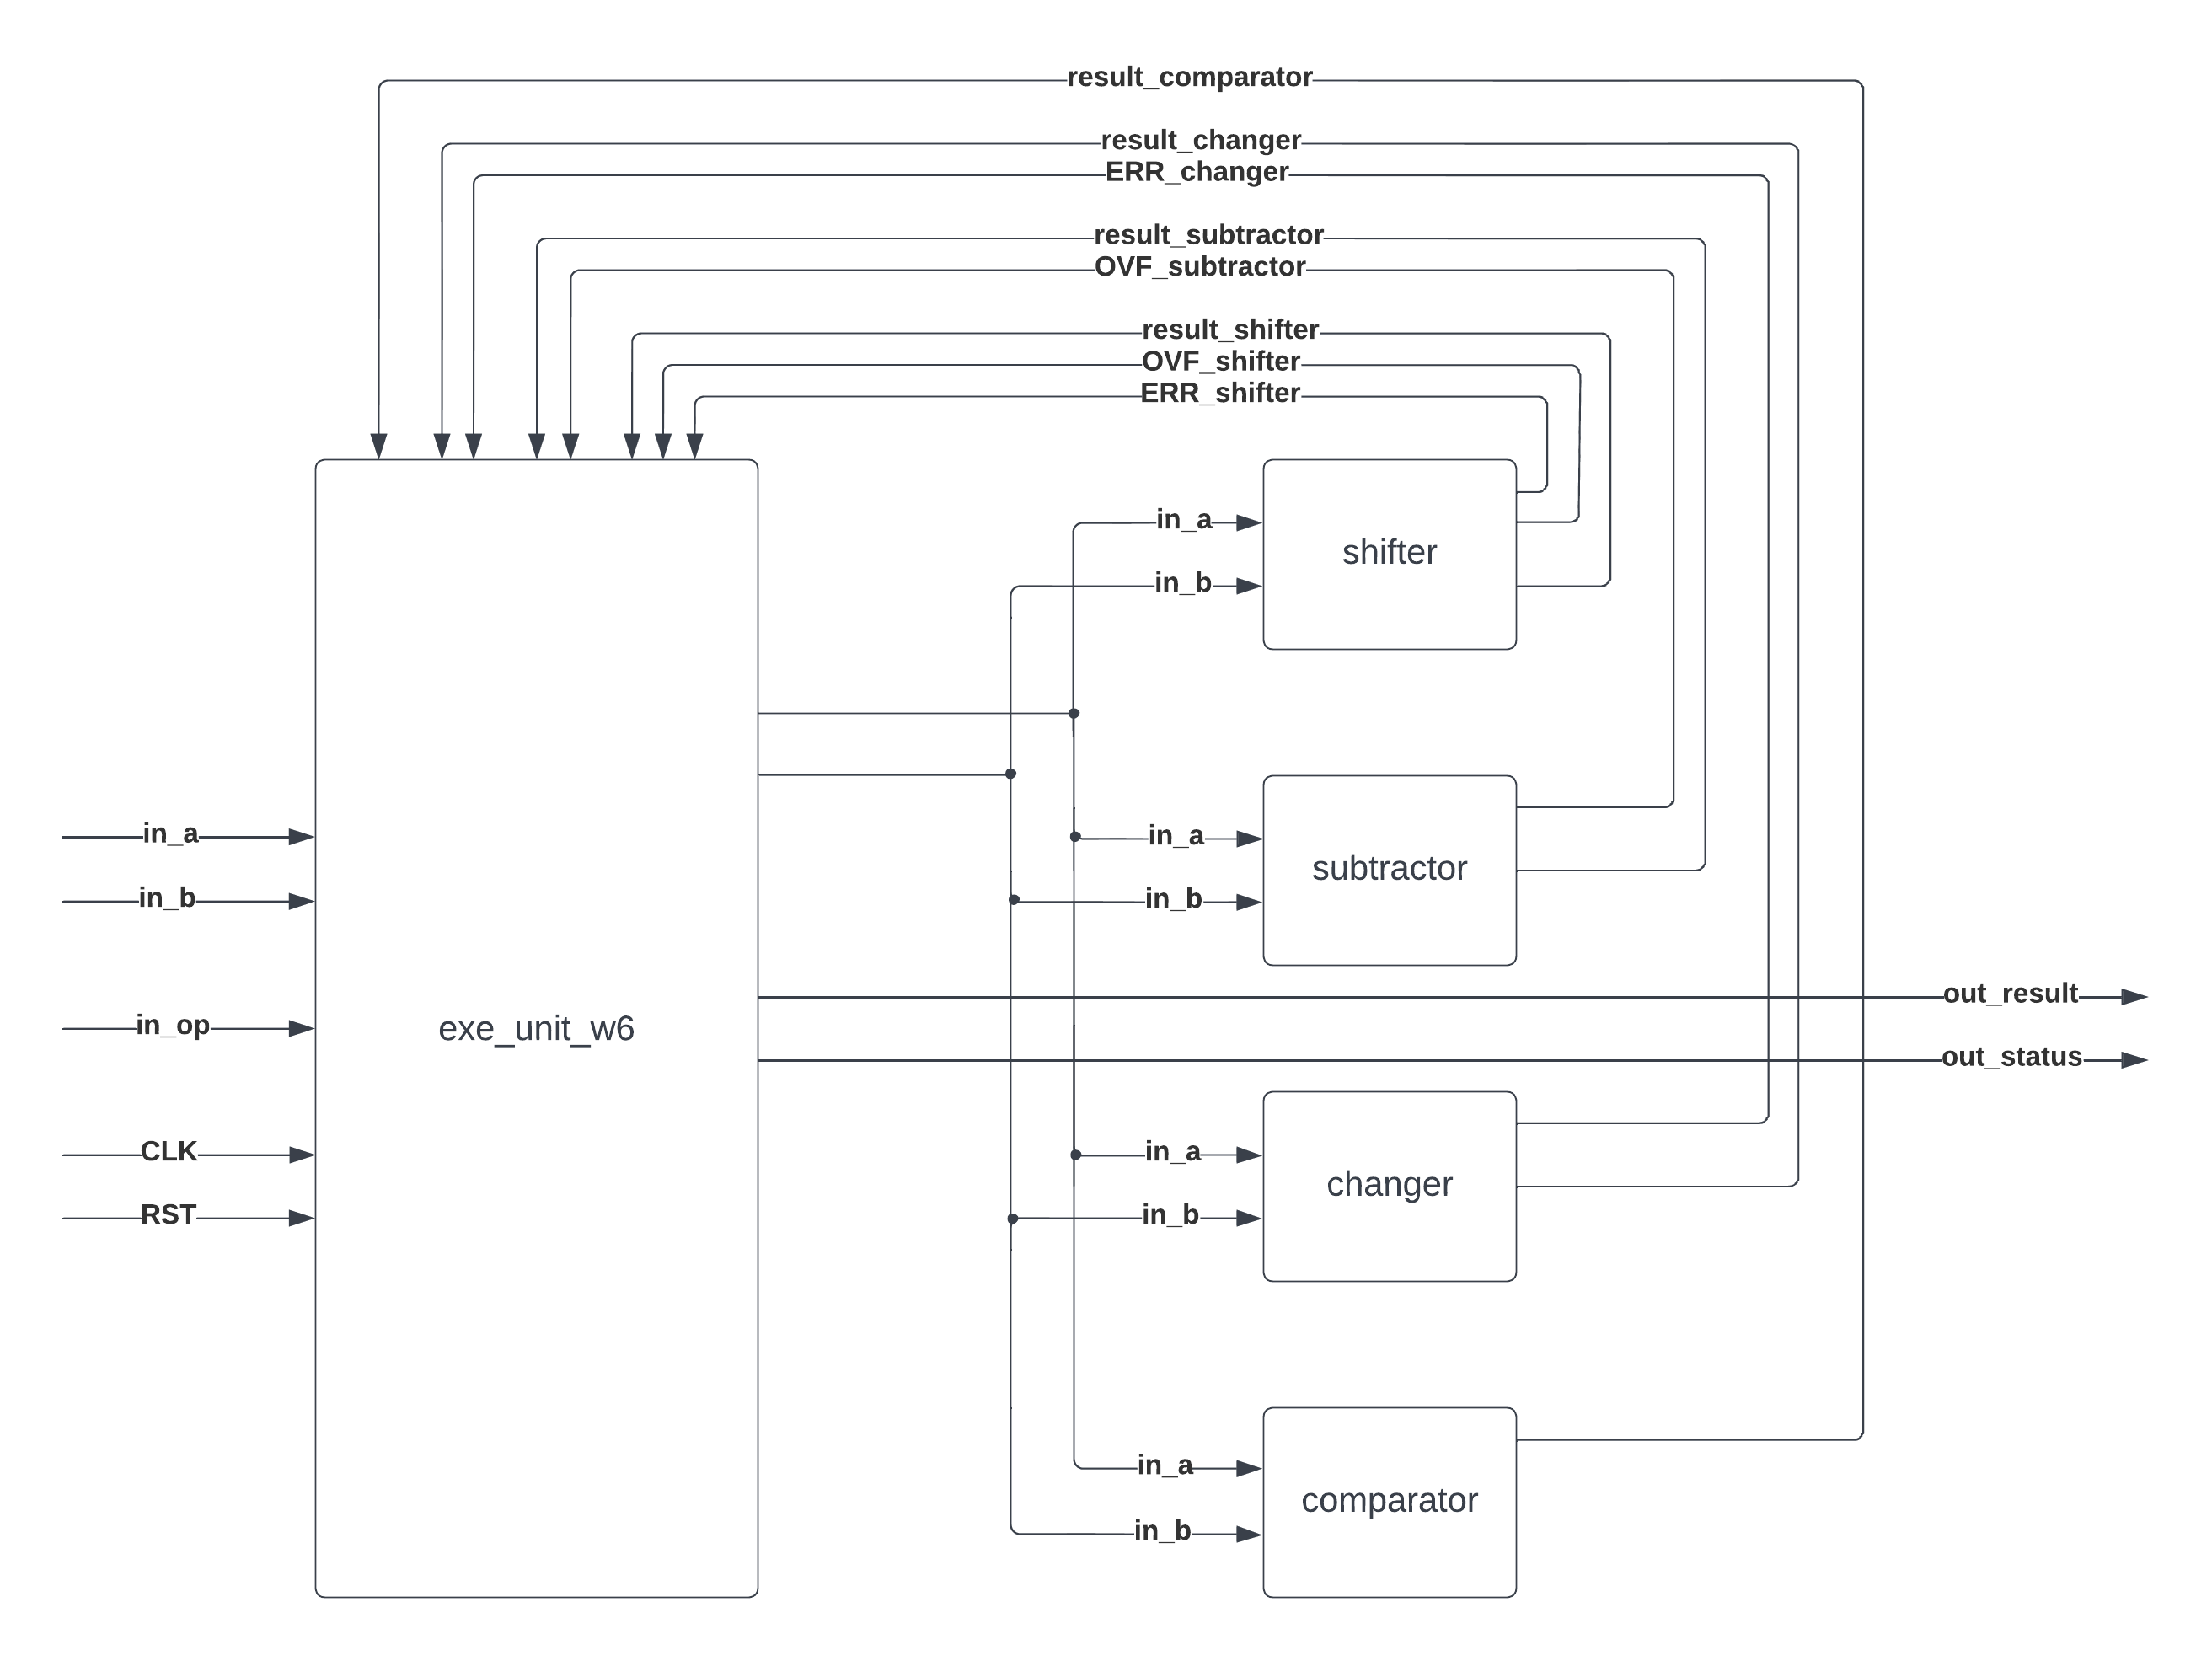
\includegraphics[width=\textwidth]{Schemat_blokowy.png}
			\caption*{Schemat blokowy jednostki \textbf{exe\_unit\_w6}}
		\end{center}
	\end{figure}
	
	
	\section*{Opis jednostki}
	Zadanie polegało na implementacji modułu \textbf{exe\_unit\_w6}. Zadaniem układu jest wykonywanie kilku zdefiniowanych operacji matematycznych i logicznych. 
	
	\subsection*{Wejścia}
	Działania są wykonywane na dwóch n-bitowych liczbach A i B (wejścia \textbf{in\_a} i \textbf{in\_b}) podanych na wejście. Wyboru operacji dokonuje się za pomocą 2-bitowego wejścia \textbf{in\_op}. Dodatkowo układ jest wyposażony w wejście zegarowe wyzwalane zboczem narastającym \textbf{CLK} i resetu synchronicznego \textbf{RST}. Stan niski na wejściu reset skutkuje przywróceniem stanu układu do stanu początkowego, czyli ustawienia operacji odejmowania dla obydwu wejść wynoszących zero. Pełna lista wejść ukłdu jest przedstawiona w Tabeli \ref{table:inputs}. Poszczególne operacje wraz z wartościami wejścia \textbf{i\_op} zostały wymienione w Tabeli \ref{table:inop_values}.  
	
		\begin{table}[!ht]
		\centering
		\begin{tabular}{|l|l|l|}
			\hline
			\textbf{Wejście} & \textbf{Funcja} & \textbf{Ilość bitów wejściowych} \\ \hline
			in\_a & Pierwszy składnik obliczeń & N-bitów \\ \hline
			in\_b & Drugi składnik obliczeń & N-bitów \\ \hline
			in\_op & Wybór operacji & 2-bity \\ \hline
			RST & Reset synchroniczny & 1-bit \\ \hline
			CLK & Taktowaniw układu & 1-bit \\ \hline
		\end{tabular}
		\caption{Lista przedstawiająca wszystkie wejścia jednostki}
		\label{table:inputs}
	\end{table}
	
	\begin{table}[!ht]
		\centering
		\begin{tabularx}{\linewidth}{|X|X|X|X|}
			\hline
			\textbf{Wartość wejścia in\_op} & \textbf{Operacja} & \textbf{Flagi wyjściowe} \\ \hline
			0b00 & Odejmowanie Liczby A od liczby B & OVF, EVEN, SINGLE \\ \hline
			0b01 & Porównanie, czy liczba \newline A >= B. Jeśli tak, to wyjście jest dodatnie. Jeśli nie to wyjście jest zerem & EVEN, SINGLE \\ \hline
			0b10 & Przesunięcie liczby A o B bitów w lewo (z zachowaniem znaku). Gdy B ma wartość ujemną lub jest większe od liczby bitów liczby A, zwróć błąd. & OVF, ERROR, EVEN, SINGLE \\ \hline
			0b11 & Zmiana bitu liczby A na pozycji B. Gdy B ma wartość ujemną lub jest większe od liczby bitów liczby A, zwróć błąd. & ERROR, EVEN, SINGLE \\ \hline
		\end{tabularx}
		\caption{Opis poszczególnych operacji wraz z kodami wejściowymi i dostępnymi flagami}
		\label{table:inop_values}
	\end{table}

	
	\subsection*{Wyjścia}
	Na wyjściu modułu dostępne są dwie wartości: \textbf{out\_result} i \textbf{out\_status}. Wyjście \textbf{out\_result} zawiera wynik ostatnio wykonywanej operacji. Na wyjściu \textbf{out\_status} pojawiają się flagi informacyjne dotyczące ostatnio wykonanej operacji. Kolejność bitów i ich funkcje zostały opisane w tabeli 2. Każda z wykonywanych operacji ma możliwość zmiany wyłącznie wybranych flag. Pełna lista wyjść znajduje się w Tabeli \ref{table:outputs}. Flagi wyjściowe z każdej operacji są zawarte w Tabeli \ref{table:outstatus_bits}. 
	
	\begin{table}[!ht]
		\centering
		\begin{tabular}{|l|l|l|}
			\hline
			\textbf{Wyjście} & \textbf{Funkcja} & \textbf{Ilość bitów wejściowych} \\ \hline
			out\_result & Wynik ostatnio wykonanej operacji & N-bitów \\ \hline
			out\_status & Rejestr z flagami infrmacyjnymi & 4-bitów \\ \hline
		\end{tabular}
		\caption{Lista przedstawiająca wszystkie wyjścia układu}
		\label{table:outputs}
		\vspace{10pt}
	\end{table}
	
	\begin{table}[!ht]
		\centering
		\begin{tabular}{l|l|l|l|l|}
			\multicolumn{1}{c}{Bit} & \multicolumn{1}{c}{3} & \multicolumn{1}{c}{2} & \multicolumn{1}{c}{1} & \multicolumn{1}{c}{0} \\ \cline{2-5}
			~ & \textbf{SINGLE} & \textbf{OVF} & \textbf{EVEN} & \textbf{ERROR} \\ \cline{2-5}
		\end{tabular}
		\caption{Bity dostępne w wektorze wyjściowym \textbf{out\_status}}
		\label{table:outstatus_bits}
	\end{table}
	
	\subsection*{Flagi}
		Rejestr wyjściowy \textbf{out\_status} składa się z 4 flag sygnalizujących stan wyjścia układu. Dodatkowo należy wspomnieć, że podczas załączenia flagi \textbf{ERROR} wyjście z układu jest nieokreślone i wynik będący wtedy na wyjściu w ogóle nie powinien być brany pod uwagę. 
		\begin{itemize}
			\item \textbf{SINGLE} - Flaga informująca, że w wyniku jest tylko jedno zero
			\item  \textbf{OVF} - Flaga informująca o przepełnienu podczas operacji
			\item  \textbf{EVEN} - Flaga informująca, że liczba zer w wyniku jest parzysta.
			\item \textbf{ERROR} - Flaga informująca o błędzie podczas wykonywania operacji.
		\end{itemize}
	
\subsection*{Instancjonowanie}

W kodzie \ref{code:instantions} pokazano ostateczne zainstancjonowanie jednostki w użyciu. W przypadku układu przed syntezą konieczne może być zdefiniowanie liczby N, czyli ilości bitów rejestrów wejściowych i wyjściowych. Wartość ta jest przechowywana w parametrze \textbf{BITS}. Nazwy podłączonych sygnałów wewnętrznych z przedrostkiem \textbf{s\_} są jedynie przykładowe i zostały użyte podczas testowania jednostki przed i po syntezie.5

\begin{program}
	\begin{verbatim}
		exe_unit_w6 #(.BITS(N_BITS)) exe_unit_w6_model (.in_a(s_a), .in_b(s_b),
	.i_op(s_op), .i_clk(s_clk), .i_rst(s_rst), .o_out(s_out_model),
	.o_status(s_status_model));    // model przed syntezą
	
	exe_unit_w6_rtl exe_unit_w6_synth (.in_a(s_a), .in_b(s_b),
	.i_op(s_op), .i_clk(s_clk), .i_rst(s_rst), .o_out(s_out_synth), 
	.o_status(s_status_synth));    // model po syntezie
	\end{verbatim}
	\caption{Przykładowe zainstancjonowanie jednostki \textbf{exe\_unit\_w6} w ostatecznym kodzie}
	\label{code:instantions}
\end{program}

	
	\section*{Opis Podmodułów}
	
	Jednostka składa się z modułu sterującego i 4 modułów wykonawczych:
	\begin{itemize}
		\setlength\itemsep{2pt}
		\item \textbf{exe\_unit\_w6} - Moduł sterujący
		\item \textbf{substractor} - Moduł odejmujący
		\item \textbf{comparator} - Moduł porównujący
		\item \textbf{shifter} - Moduł wykonujący operację przesunięcia
		\item \textbf{changer} - Moduł zmieniający bit na 1 na danej pozycji
	\end{itemize}
	Każdy z modułów wykonawczych odpowiada za daną operację. Z podmodułów wychodzą sygnały zawierające wynik operacji i ewentualne flagi informacyjne. W module sterującym wchodzą one do multipleksera, który podaje na wyjście wynik wybranych flag i operacji.
	
	\section*{Synteza logiczna}
	
	\subsection*{Raport z syntezy}
	Pełny raport z syntezy znajduje się w pliku \textbf{Pliki\_projektu/synth.log}
	\section*{Symulacja i testy}
	\section*{Struktura plików}
	
\end{document}